\documentclass{article}

% Packages
\usepackage{graphicx} % For including images
\usepackage{amsmath} % For mathematical symbols and equations
\usepackage{hyperref} % For hyperlinks
\usepackage{listings} % For including code snippets
\usepackage[ngerman, american, british, UKenglish, USenglish]{babel} %For spellchecking
\usepackage{microtype}
\usepackage[a4paper, total={6in, 9in}]{geometry}
%\setlength{\columnsep}{20pt}
\usepackage{float}



\title{Exposé: Bachelor Thesis about the creation of a device to perform wireless cyber attacks on}
\author{Jonas Schmitt}
\date{\today}

\begin{document}

\maketitle

\section{Introduction}

The modern world is moving towards digitalization at a high pace, which aims to make it smart and interconnected. Therefore there's an increasing number of IoT(Internet of Things) devices, 
which are connected to the internet or use some sort of wireless communication.
Because these devices oftentimes are essential for our daily lives and in case of our phones and computers contain some of our most valuable data, it is essential to keep them secure.
In order to assess the security of a technology, penetration testing is used to discover weaknesses in soft- and hardware, which could be exploited by malicious actors.
The goal of this bachelor thesis is to create a device, which can easily be set up and attacked in order to test out various attacks on wireless communication and web applications.  

\section{Devices}

The device will be created, using a Raspberry PI 4 (RPI) single board computer and an ESP32 Microcontroller. 
The RPI has a quad core ARM CPU, 8GB of RAM and comes equipped with a network chipset for WIFI AC as well as Bluetooth 5.0/LE. 
For setting up a hotspot with WPA3 encryption, the internal WIFI chipset cannot be used, therefore an extra external WIFI adapter is necessary.
The ALFA AWUS036AXM USB WIFI adapter was chosen for optimal compatibility with the Linux Kernel and availability of information.
Furthermore the board can be connected to expansion cards for e.g. NFC or RF communication.
As a communication partner for the RPI an ESP32-WROOM-32 Chipset by Espressif is used. The ESP32 comes on a generic development board and offers a radio for WIFI as well as Bluetooth LE.
With it's low power RISC-V processor and 4MB of flash memory, the ESP32 offers a cost effective platform for IoT applications, for which it is commonly used. 



\section{Goals}

The general goal is to create an application in C++ with a simple command line interface, like the concept depicted in the following image:

\vfill

\begin{figure}[H]
    \centering
    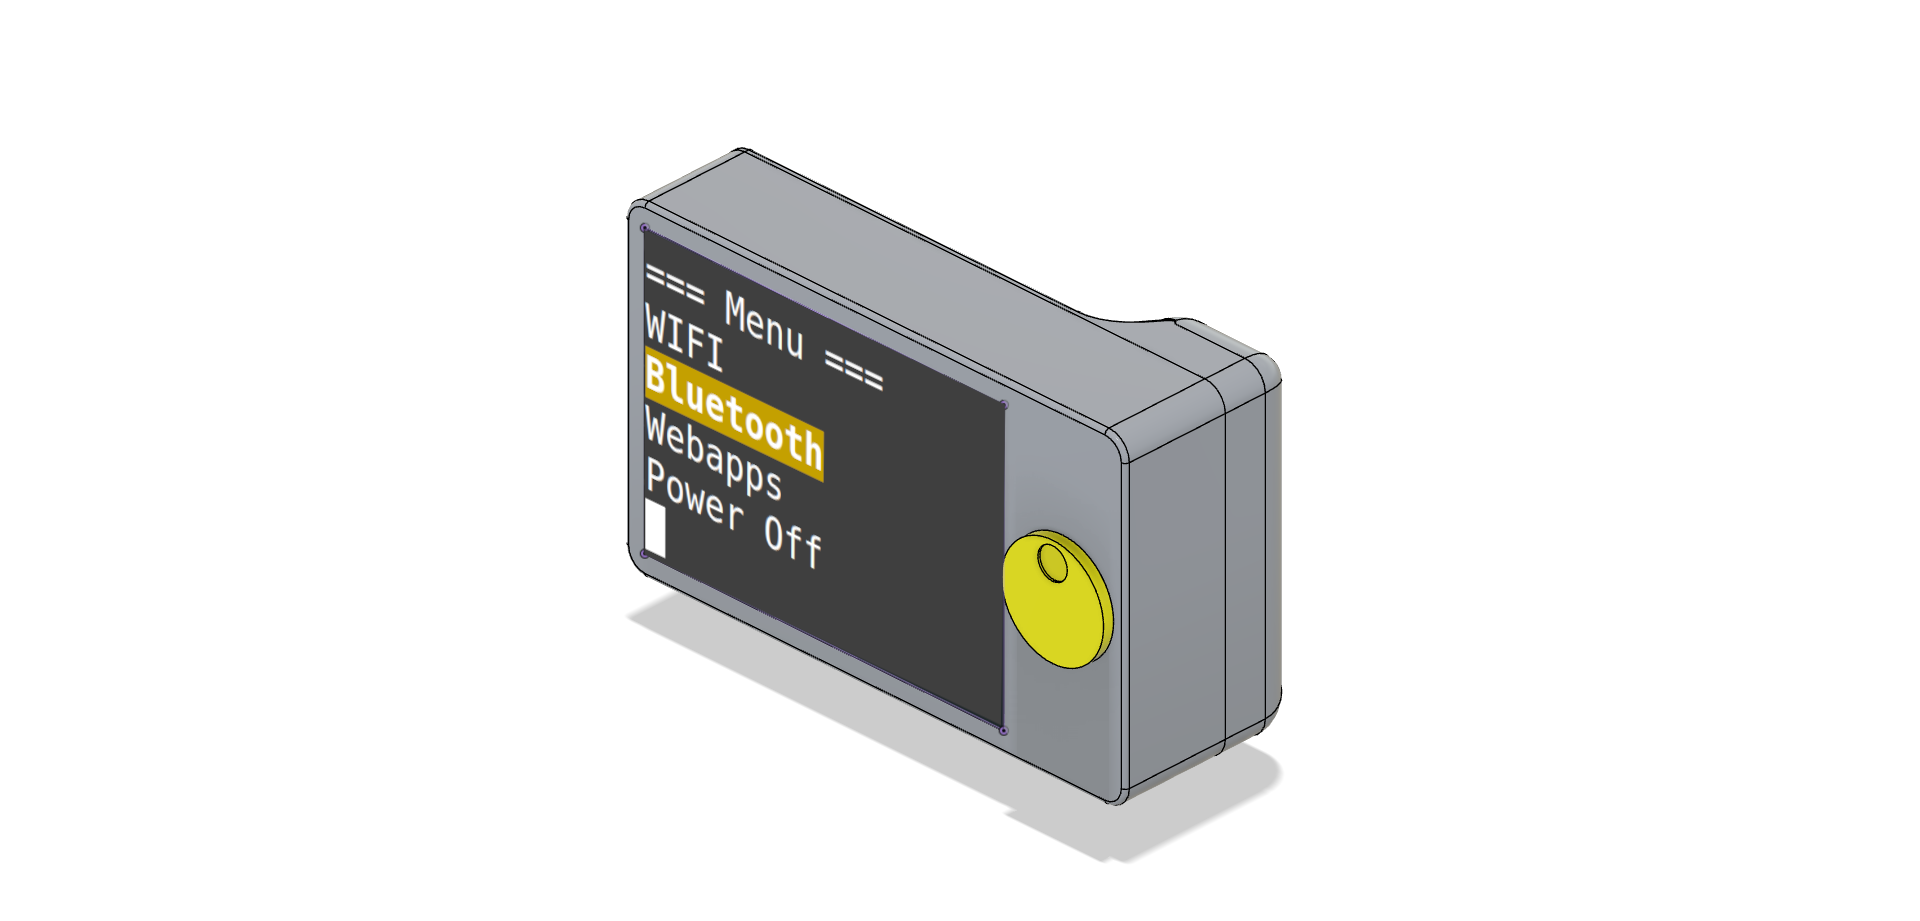
\includegraphics[width=\columnwidth]{Concept.png}
    \caption{Device Concept}
    \label{fig:image1}
\end{figure}

The UI application allows the execution of shell scripts in order to configure the RPI for the following scenarios:

\begin{itemize}
	\item opening a hotspot on the RPI with a known SSID and password, launching the OWASP juice shop project for testing exploitation of vulnerabilities in web applications 
	\item opening a hotspot on the RPI with either a random SSID/password and WEP encryption or WPA/WPA2/WPA3 encryption with a configurable password. 
    Starting unencrypted MQTT communication between RPI and ESP32. 
    The attacker can try to crack the WIFI password and read the traffic between the RPI and ESP32. 
    The process of the attack, e.g. the fake authentication, deauthentication of the ESP32, receipt of an IP address, snooping, etc. should be tracked by the RPI 
    \item activating Bluetooth, optionally turning on discovery mode, creating a dummy "sensitive information" file. The attacker can try to perform the "BlueSnarf" attack. 
    The process of the attack should be tracked by the RPI.
	\item pairing to the ESP32 via Bluetooth, creating dummy traffic. The attacker can try to perform the "BlueDump" attack.
    The process of the attack should be tracked by the RPI.
	\item resetting all previously made changes
	\item optional: setting up the RPI for NFC attacks
	\item optional: setting up the device to try exploitation of vulnerabilities in old software releases, e.g. "BlueBourne" attack 
\end{itemize}

A user manual, containing information on setup and operation of the device will be created and appended to the thesis.


\section{Optional Features}
    If spare time is available, the following features will (partially) be implemented:

    \begin{itemize}
        \item optional points in "Goals"
        \item conversion to battery power
        \item use of a more efficient SBC than the RaspberryPI 4
    \end{itemize}

\section{Similar works}
Upon online research, a similar project could not be found.


\section{Structure}

the structure of the thesis is not clear yet, but could look like the following:

\begin{enumerate}
    \item Introduction
    \item Content
    \begin{enumerate}
        \item Importance of security in wireless communication
        \item Vulnerabilities in WIFI and Bluetooth
        \item device presentation
        \item list of possible attacks and according tests
    \end{enumerate}
    \item Conclusion
    \begin{enumerate}
        \item Educational benefits
        \item Research benefits
    \end{enumerate}
    \item Appendix
    \begin{enumerate}
        \item user manual
    \end{enumerate}
\end{enumerate}

\section{Schedule}

The coding of the UI application and shell scripts should be finished until the end of 2024. Research and writing of the thesis will be performed in parallel. 
In January and February of 2025 the thesis shall receive its finishing touches.


\section{Sources}

\begin{itemize}
    \item \href{https://www.makeuseof.com/bluetooth-attacks/}{11 Bluetooth Attacks You Need to Know About by Fatih Küçükkarakurt}
    \item \href{https://github.com/morrownr/USB-WiFi/blob/main/home/USB_WiFi_Adapters_that_are_supported_with_Linux_in-kernel_drivers.md}{USB WiFi Adapters that are supported with Linux in kerneldrivers}
    \item \href{https://forums.raspberrypi.com/viewtopic.php?t=364824#}{Raspberry PI 4 WPA3 support}
    \item \href{https://www.w3schools.com/cybersecurity/cybersecurity_wifi_attacks.php}{WIFI Attacks}
    \item \href{https://learning.oreilly.com/course/wifi-hacking-wireless/9781789530193/}{WiFi Hacking: Wireless Penetration Testing for Beginners}
    \item \href{https://www.kali.org/tools/}{Kali Tools}
    \item \href{https://link-springer-com.thn.idm.oclc.org/book/10.1007/978-3-642-40646-1}{Bluetooth security attacks : comparative analysis, attacks, and countermeasures}
    \item \href{https://help.owasp-juice.shop/}{Pwning OWASP Juice Shop by Björn Kimminich}
\end{itemize}



\end{document}
